%----------------------------------------------------------------------------
\chapter{\bevezetes}
%----------------------------------------------------------------------------

\section{Motivation}

The navigation of mobile robots has been a dynamic area of research, with significant advancements worldwide. For autonomous vehicles to perform their tasks efficiently, it is crucial that they first explore and understand their surroundings. Without a structured approach to navigation, these robots risk becoming lost or colliding with obstacles in their environment.

One familiar example of an autonomous agent is the robot vacuum cleaner. I have firsthand experience with two models: an older iRobot Roomba 780, which I own, and a newer iRobot Roomba i7, which belongs to my parents. The Roomba 780, released in 2010, operates on a simpler navigation approach. It moves from wall to wall and lacks the ability to localize or map its environment, and relies solely on wheel rotation measurements for movement tracking. When it encounters an object, it changes direction and continues its sweeping path.

By contrast, the Roomba i7 integrates a low-resolution camera on its top, which captures small images of the ceiling for spatial awareness while respecting privacy constraints. On its first run, the i7 initiates an autonomous mapping process, moving systematically through rooms to build a map of the space. Once mapping is complete, users can view the apartment layout in a companion app. This model offers significant improvements over the 780: it can locate its docking station, recognize individual rooms, and localize itself within the apartment, allowing it to clean methodically and efficiently.
\FloatBarrier
\begin{figure}[htbp]
	\centering
	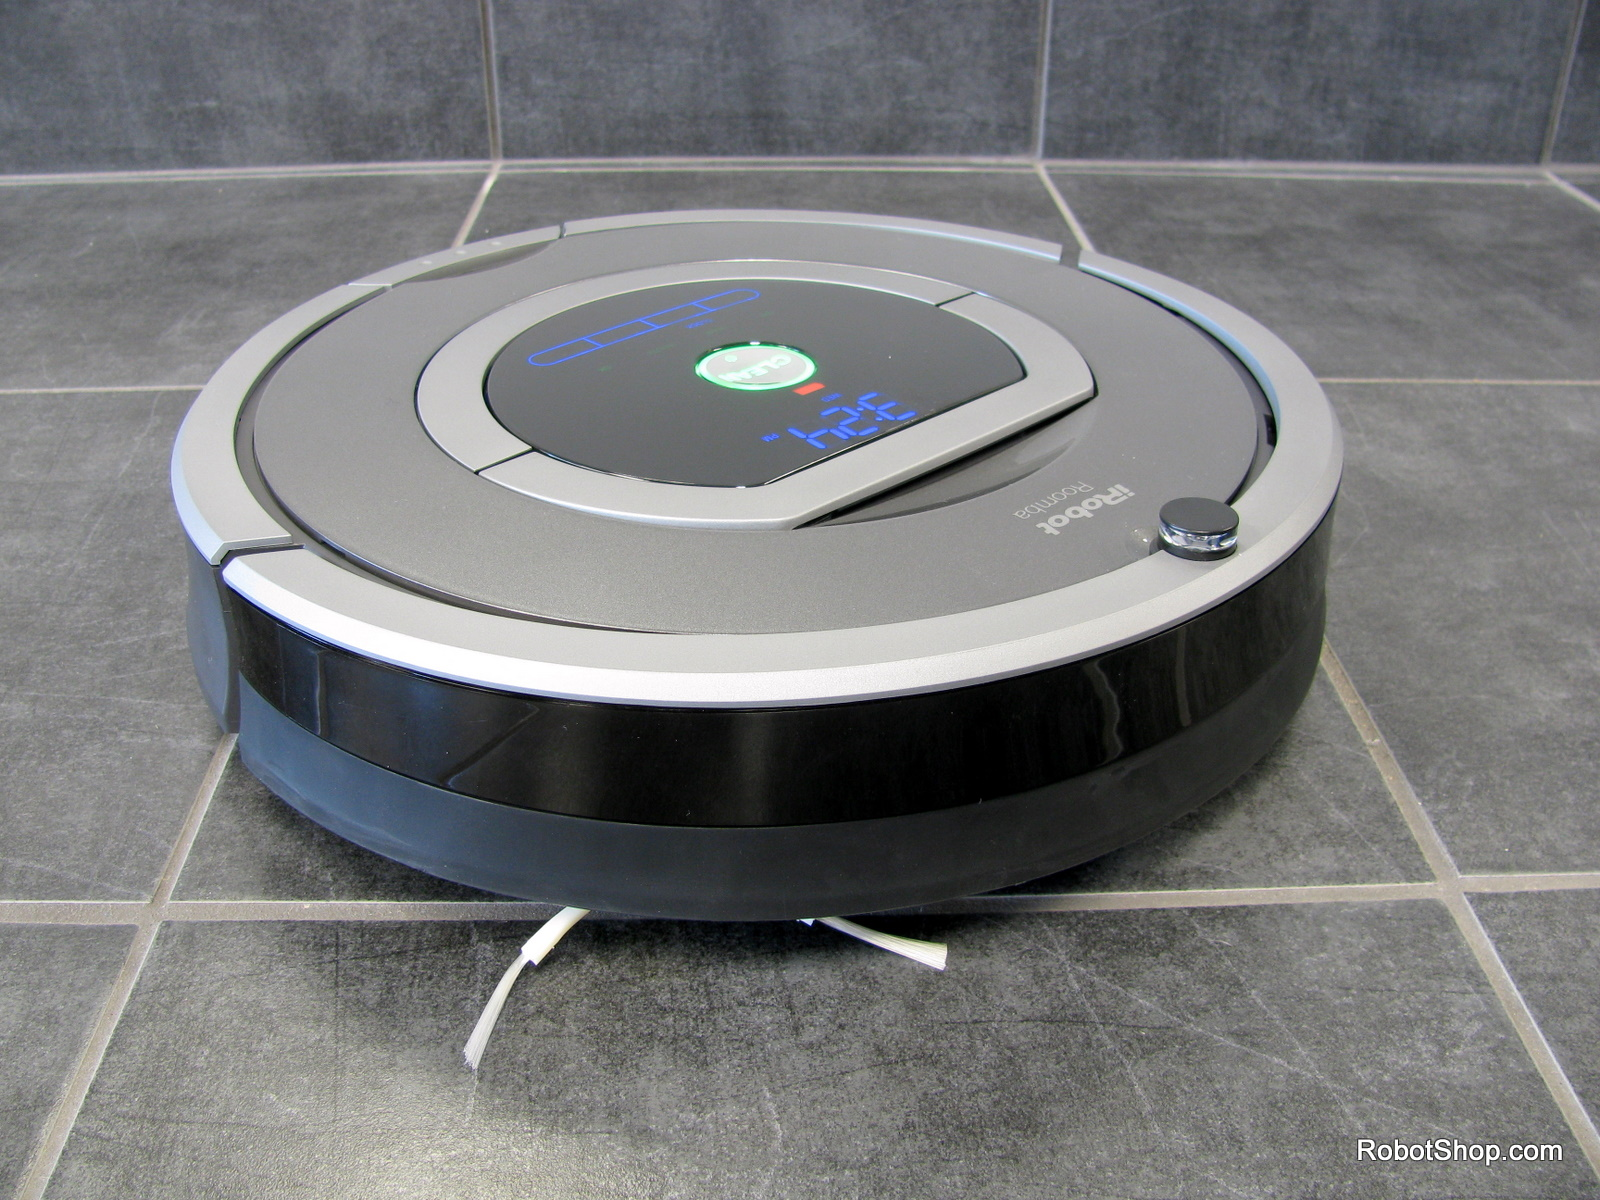
\includegraphics[width=67mm, keepaspectratio]{figures/iRobot_roomba_780.jpg}\hspace{1cm}
	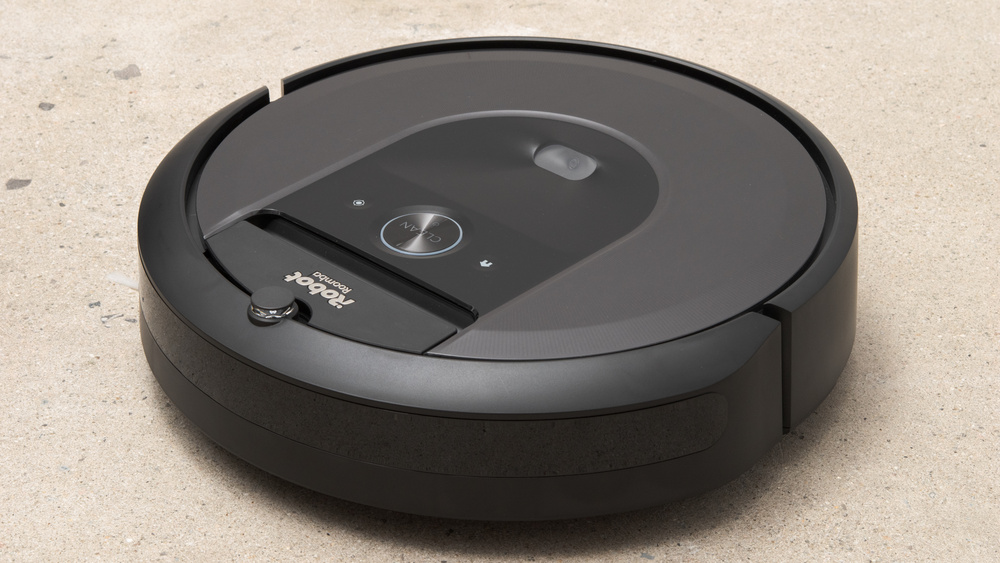
\includegraphics[width=67mm, keepaspectratio]{figures/iRobot_roomba_i7.jpg}\\\vspace{5mm}
	\caption{Robot vacuum cleaners iRobot Roomba 780 (left) and i7 (right), sources: \cite{roomba780}\cite{roombai7}}
	\label{fig:Roombas}
\end{figure}
\FloatBarrier
This example highlights the advantages of simultaneous localization and mapping (SLAM) in a household environment. SLAM technology is also transformative in industrial contexts. For instance, autonomous robots can transport heavy products across large warehouses. In such scenarios, a wall-to-wall navigation algorithm would be impractical, as it would likely fail to reach its destination before depleting its battery. Consequently, modern autonomous systems increasingly rely on SLAM algorithms to enable efficient and reliable navigation.

In industrial settings, autonomous robots are evolving beyond simple navigation tasks to handle more complex activities, such as moving and organizing inventory. As illustrated in Figure~\ref{fig:robots_in_warehouse}, robots equipped with manipulators can load packages onto mobile robots that transport items across warehouses. These combined systems of robotic arms and mobile platforms represent a new frontier for industrial automation, where robots can not only navigate large spaces but also carry out detailed, repetitive tasks that require precise movements and lifting capabilities. This level of automation has the potential to significantly increase operational efficiency, reduce human labor in hazardous or strenuous tasks, and streamline the logistics of large-scale storage and distribution.

\FloatBarrier
\begin{figure}[htbp]
	\centering
	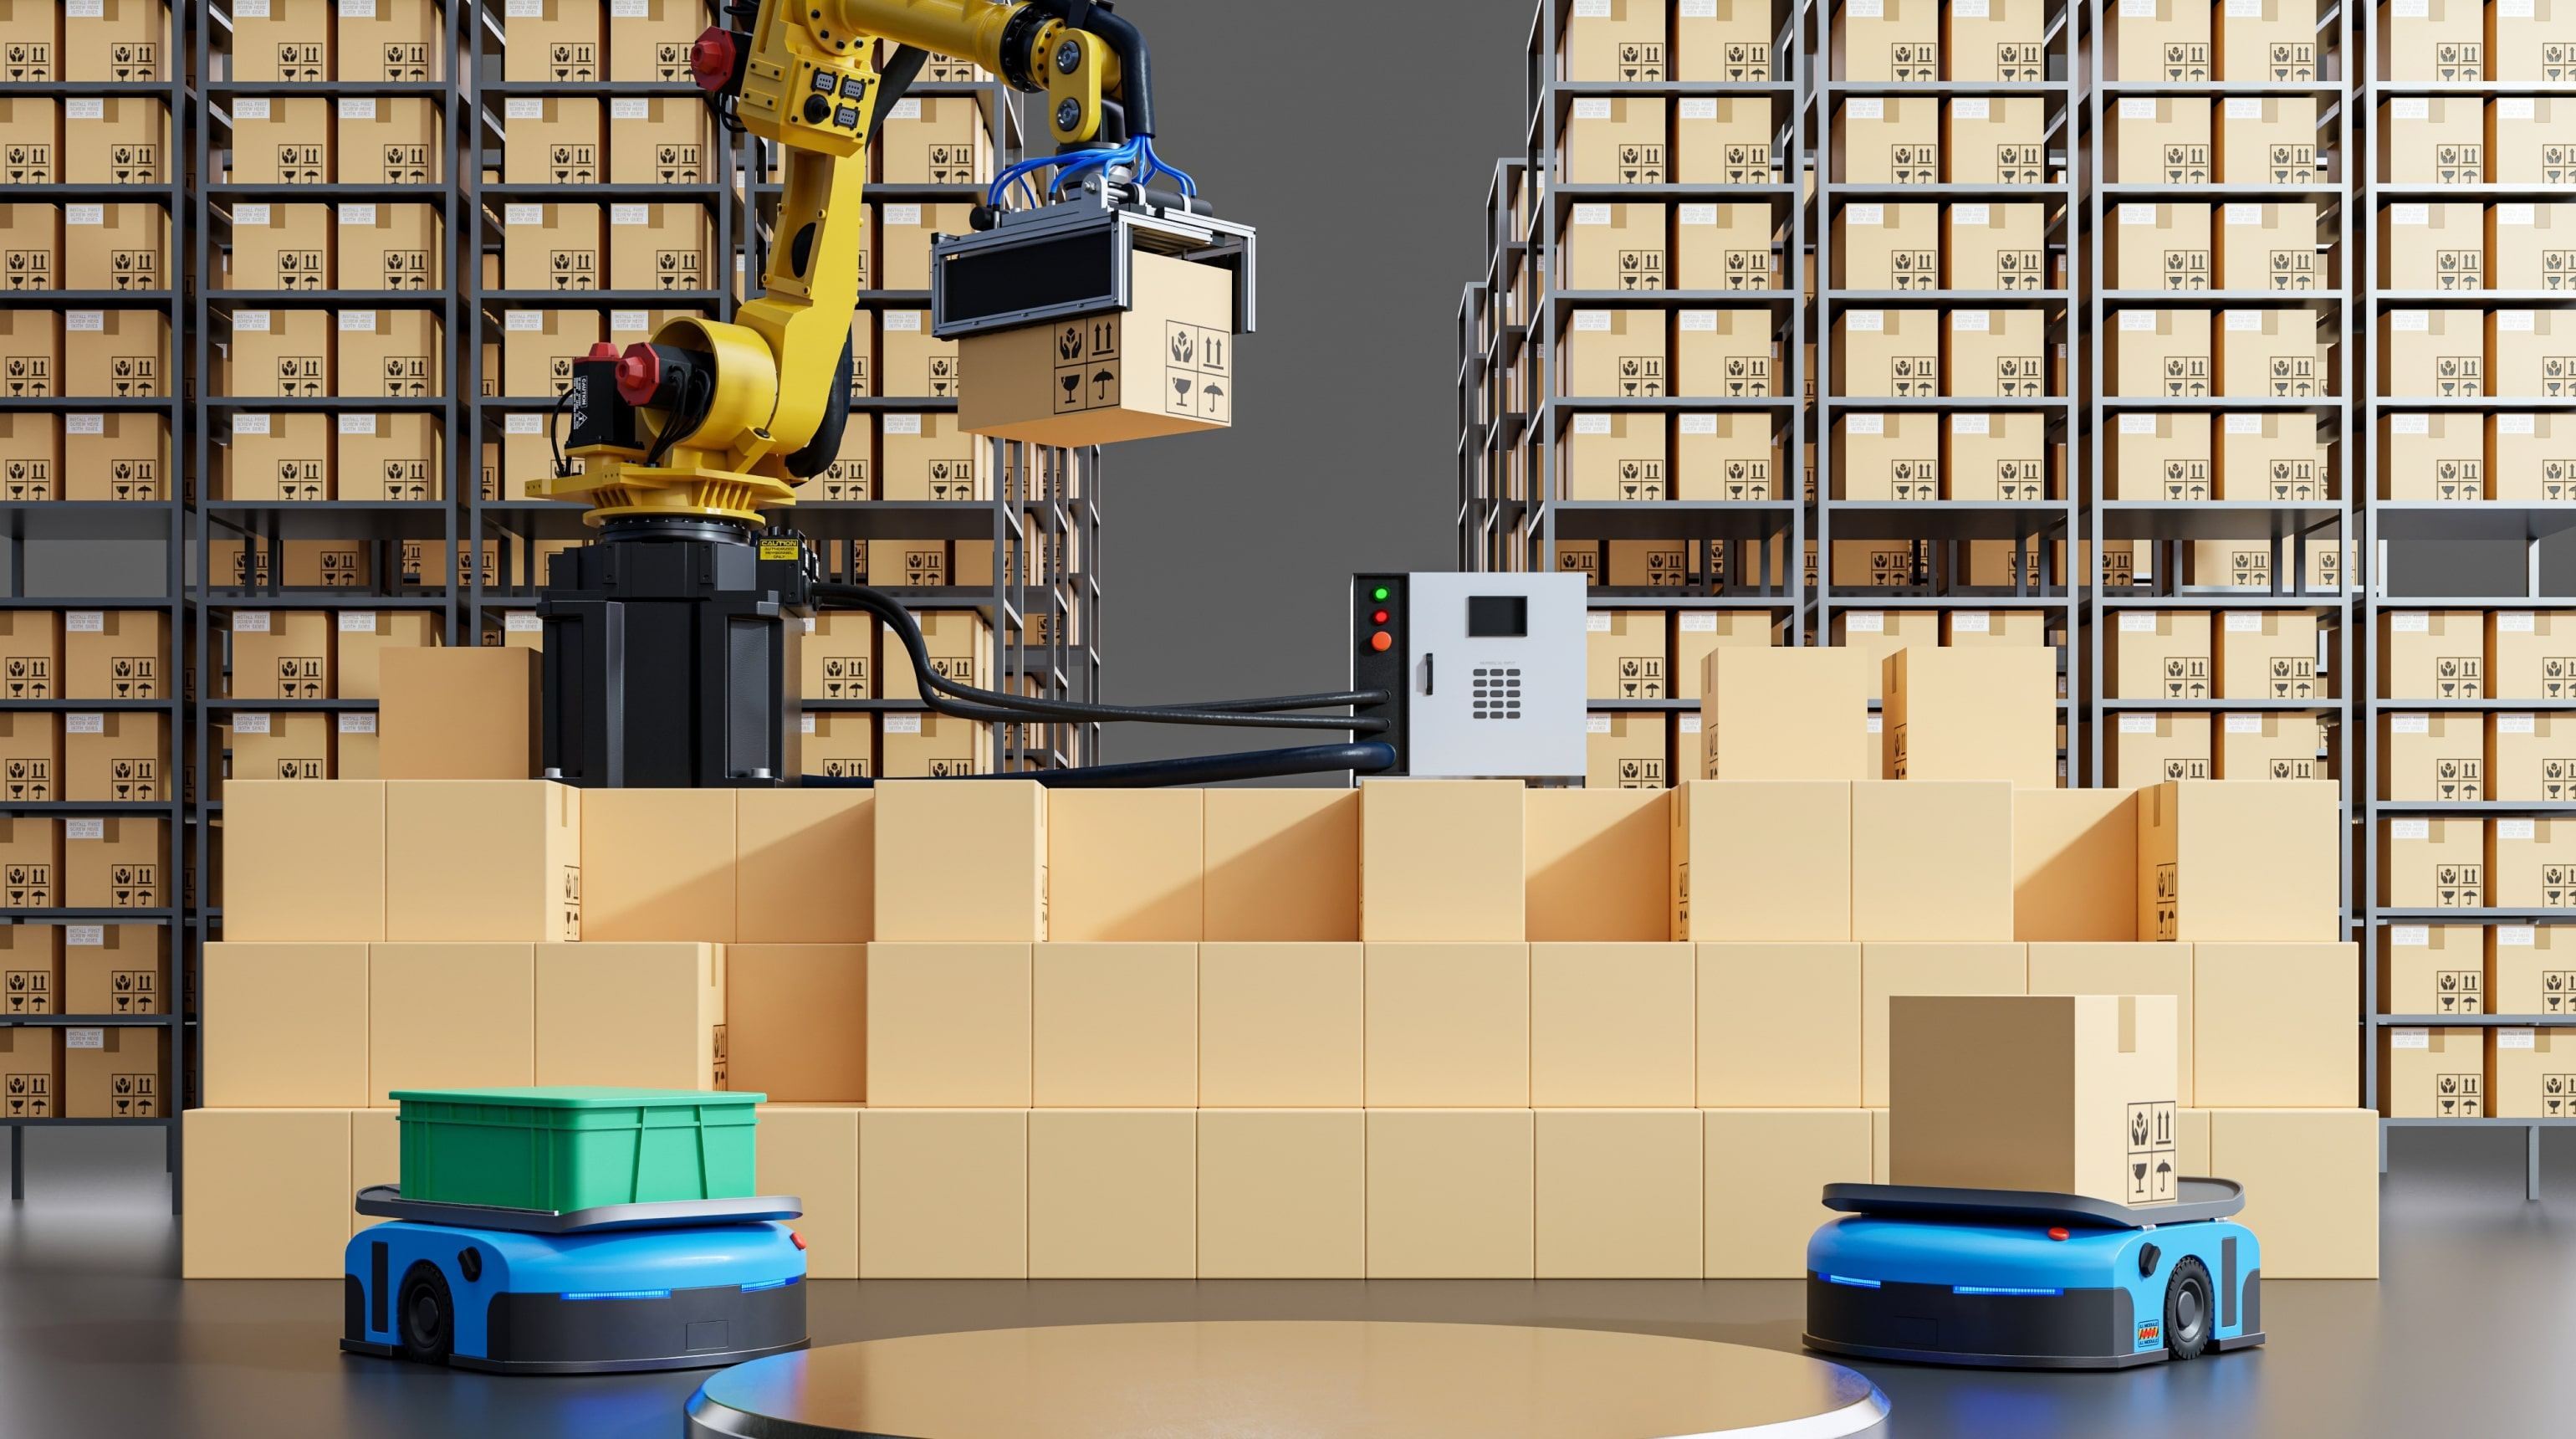
\includegraphics[width=150mm, keepaspectratio]{figures_jpg/warehouse_robots.jpg}
	\caption{Illustration of robots used in a warehouse, source:~\cite{robots_in_warehouse}}
	\label{fig:robots_in_warehouse}
\end{figure}
\FloatBarrier

In summary, SLAM plays an essential role in empowering mobile robots to understand and navigate their environments effectively, whether in homes or complex industrial settings.

Mobile robotics technology may one day extend to fully autonomous household assistants, as illustrated in Figure~\ref{fig:futuristic_house_cleaning_robot}. This concept envisions a future where robots with manipulators, or robotic "hands" perform routine household chores, such as loading the dishwasher or organizing items~\cite{physical_intelligence}. The development of such robots could revolutionize domestic life by reducing the time and effort spent on daily tasks, enabling greater convenience and flexibility for homeowners. As mobile robots become capable of not only navigating but also manipulating their environment, they have the potential to transform lifestyles, adding a new dimension to household automation and creating more time for people to engage in other activities.

\FloatBarrier
\begin{figure}[htbp]
	\centering
	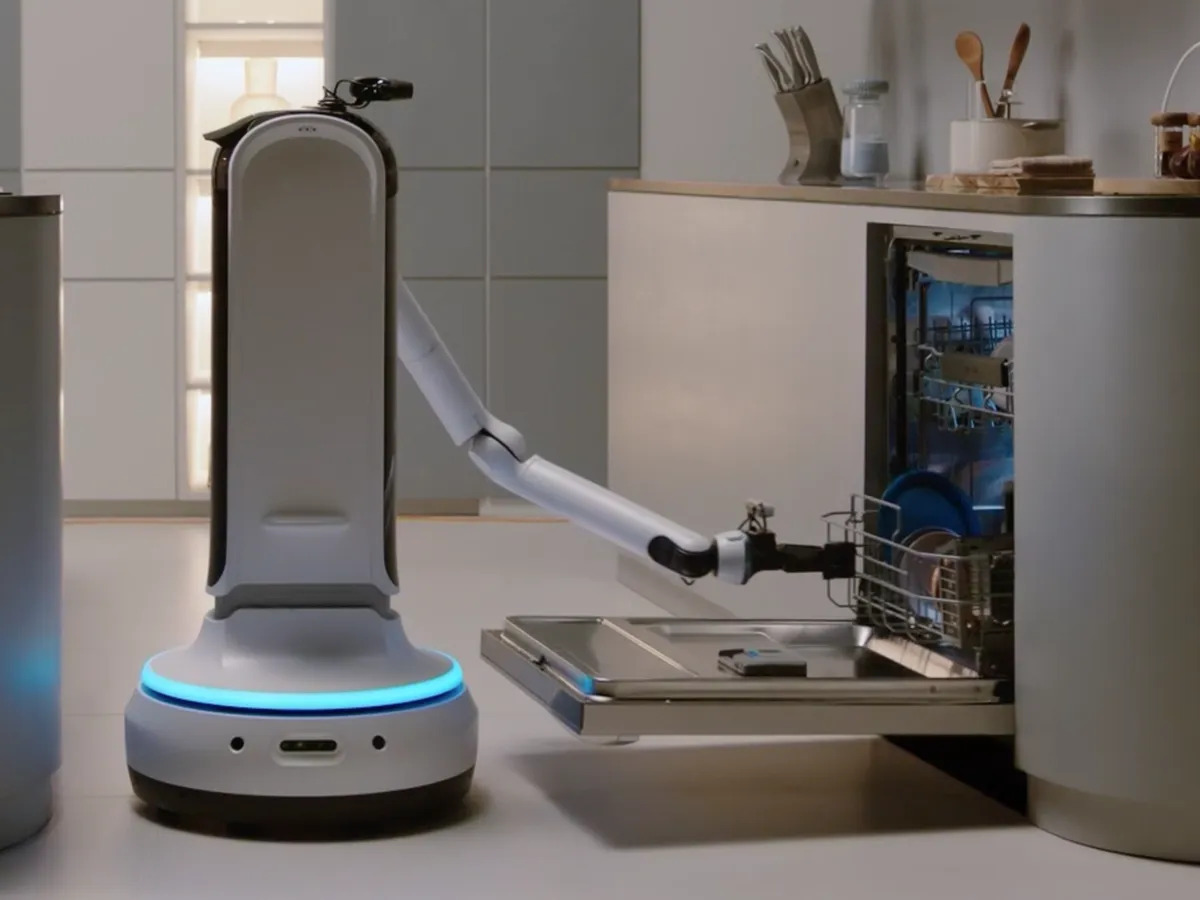
\includegraphics[width=150mm, keepaspectratio]{figures_jpg/samsung-bot-handy.jpg}
	\caption{A futuristic house cleaning robot, source:~\cite{futuristic_household_robot}}
	\label{fig:futuristic_house_cleaning_robot}
\end{figure}
\FloatBarrier

\section{Goal of the thesis}

The primary objective of this thesis is to advance the exploration and mapping capabilities of a (Roomba-like) mobile robot, enabling it to map new environments. The resulting map can then be reused by the robot itself or shared with other robots, supporting coordinated navigation and interaction in shared spaces.

The main focus of this work is to implement Visual SLAM (V-SLAM) using a stereo camera, as opposed to traditional SLAM methods that rely on LiDAR. Stereo cameras can capture detailed 3D maps or point clouds, enhancing the robot's spatial awareness.

In addition to these core objectives, two optional goals were pursued:
\begin{itemize}
\setlength\itemsep{0em}
    \item Person detection and tracking: Using the camera to identify and track people, allowing the robot to either follow or avoid them as needed.
    \item Photorealistic scene reconstruction: Generating high-quality, realistic representations of the environment for advanced visualization.
\end{itemize}

Through these goals, this thesis aims to enhance the utility, versatility, and adaptability of mobile robots in various environments by leveraging advanced V-SLAM techniques.


\section{Structure of the project and the thesis}

During the writing of my thesis, I have gained significant experience in many fields. First, I learned about the scientific background of mobile robotics, their odometry, localization, mapping, SLAM and photorealistic reconstruction, which I present in Chapter~\ref{background}. Then, I learned about the Robot Operating System, the robot used at Nokia Bell Labs, OAK-D cameras, neural reconstruction and different types of 3D mapping in Chapter~\ref{related_works}. After, I digged deeper in the capabilities of the OAK-D camera in Chapter~\ref{experiments_oak_d}, experimented with 3D mapping using RTAB-Map, nvblox and Isaac VSLAM in Chapter~\ref{experiments_3d_mapping}, and gained experience in photorealistic reconstruction with NeRFs and Gaussian Splatting in Chapter~\ref{nerf_gsplat}. Then, I implemented an end-to-end mapping and photorealistic reconstruction pipeline which is presented in Chapter~\ref{implementation}. I evaluated the reconstruction pipeline in Chapter~\ref{evaluation}, and I summarized the achievements of this thesis in Chapter~\ref{summary}.
